\documentclass{article}

\usepackage[final]{neurips_2019}

\usepackage[utf8]{inputenc}
\usepackage[T1]{fontenc}
\usepackage{hyperref}
\usepackage{url}
\usepackage{booktabs}
\usepackage{amsfonts}
\usepackage{nicefrac}
\usepackage{microtype}
\usepackage{graphicx}
\usepackage{xcolor}
\usepackage{lipsum}

\newcommand{\note}[1]{\textcolor{blue}{{#1}}}

\title{
  Whisky GPTaster \\
  \vspace{1em}
  \small{\normalfont Stanford CS224N Custom Project}  % Select one and delete the other
}

\author{
  Akram Sbaih \\
  Department of Computer Science \\
  Stanford University \\
  \texttt{akram@stanford.edu} \\
  % Examples of more authors
%   \And\\
%   Name \\
%   Department of Computer Science \\
%   Stanford University \\
%   \texttt{name@stanford.edu} \\
%   \And
%   Name \\
%   Department of Computer Science \\
%   Stanford University \\
%   \texttt{name@stanford.edu}
}

\begin{document}

\maketitle

% \begin{abstract}
%   Required for final report
% \end{abstract}


%\note{This template is built on NeurIPS 2019 template\footnote{\url{https://www.overleaf.com/latex/templates/neurips-2019/tprktwxmqmgk}} and provided for your convenience.}

\note{I still have no mentor for this project.}

%\section{Key Information to include}
%
%\begin{itemize}
%    \item External collaborators (if you have any):
%    \item Mentor (custom project only):
%    \item Sharing project:
%\end{itemize}


\section{Research paper summary}

\begin{table}[h]
    \centering
    \begin{tabular}{ll}
        \toprule
        \textbf{Title} & Generating Sentiment-Preserving Fake Online Reviews Using Neural \\ &  Language Models and Their Human- and  Machine-based Detection \\
        \midrule
        \textbf{Authors} & David Ifeoluwa Adelani,  Haotian Mai,  Fuming Fang,  Huy H. Nguyen,  \\& Junichi Yamagishi,  Isao Echizen \\
        \textbf{Venue} & Advanced Information Networking and Applications -- AINA \\
        \textbf{Year}  & 2020 \\
        \textbf{URL}   & \url{https://arxiv.org/abs/1907.09177} \\
        \bottomrule
    \end{tabular}
    \vspace{1em}
%    \caption{Sample table for bibliographical information~\cite{rajpurkar2018know}.}
\end{table}

\paragraph{Background.}$ $
%Set the scene for the paper, looking to the introduction section, as well as the related work or background sections, if they exist.
%What motivations and problems do the authors cite when explaining why they think this work is important? 
%What problems are they attempting to solve, or what knowledge are they hoping to discover?
\\\\ The authors point out the huge implications of reviewes on businesses in our online world given their status as a reference for potential new clients. They cite research showing how the business could gain big profits or suffer losses as the result of a mass review attack on their products.  To be able to detect and stop such attacks,  the authors pursue a better understanding of powerful methods to generate fake reviews.
\\\\ In their discussion of related works,  they talk about techniques like manual generation and basic language model (LSTM-based) utilization.  The former is too expensive while the latter requires post-processing to make its results centered around the business attacked (to stay on topic).  They also mention the recent introduction of more sophisticated language models like GPT-2 and BERT and their advantages of pre-training and fine-tuning leading to more consistent generation of longer sequences.  
\\\\ The authors use these points to motivate their goal of using GPT-2 and BERT to generate fake reviewes of a given  sentiment for a given business with minimal human internvention.  Concretely,  they want the model to take an example review for a business, and generate a pool of fake reviews describing the same business with the same sentiment.  They also want to evaluate existing machine and human techniques on distinguishing these fake reviews from real ones.
\paragraph{Summary of contributions.}$ $
%Each paper is published because it adds something to the ongoing research conversation. It teaches us something we didn't know before, or provides us with a tool we didn't have, etc.
%Summarize what contributions this paper makes, whether they be in new algorithms, new experimental results and analysis, new meta-analysis of old papers, new datasets, or otherwise.
\\\\ The authors implemented their novel algorithm as shown in Figure~\ref{Fig:fake_review_attack}.  It consists of a generation step that takes a sample existing review as a seed,  and employs GPT-2 to generate a new fake one.  After that,  BERT is used in the validation step to find the sentiment of the fake generation and compare it to the sentiment of the original review.  This way,  BERT filters out all bad generations that have mismatching sentiment as desired. 
\\\\ They use the pretrained version of GPT-2 (with 117M parameters) and BERT and fine-tune them on positive and negative real reviews from Amazon and Yelp (they don't disclose the size of these datasets).  No pre-processing is done except concatenating all the reviews into one huge text file separated by new lines and shuffled on sentiment.  After fine-tuning,  GPT-2's generation started looking more like reviews and BERT achieved 96\% accuracy on positive/negative sentiment classification on the test set.    
\\\\ Furthermore,  human and machine evaluation were mostly incapable of distinguishing fakes from reals.  The subjective evaluation by 80 humans showed that they pointed out fake reviews at random while machines (Grover,  GLTR,  and OpenAI GPT-2 detector) showed similar behavior.
\begin{figure}[tb]
 \centering
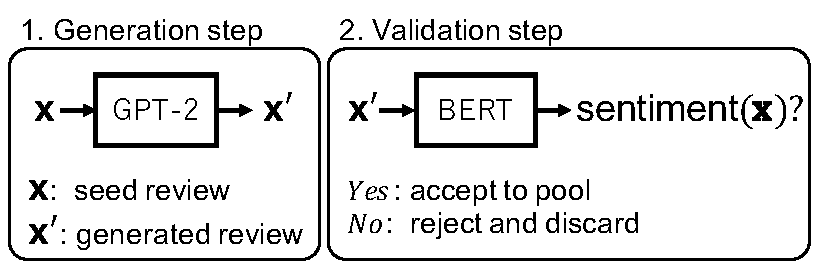
\includegraphics[width=0.7\columnwidth]{approach.pdf}
\vspace{-4mm}
\caption{Fake review generation procedure}
\label{Fig:fake_review_attack}
\vspace{-3mm}
\end{figure}
\paragraph{Limitations and discussion.} $ $
%Every research paper has limitations and flaws.
%Using the discussion and conclusion sections if they exist, critically identify interesting experiments, methodology, or methods that might have made this paper stronger.
%For example, did the authors only evaluate on English, or only on Wikipedia text, and claim that their results generalize to all of language?
%Did the authors not characterize the errors their model makes compared to previous models?
%Discuss how these limitations contextualize the findings of the paper -- do you still find the paper convincing?
\\\\ Reviewes tend to be similar in their content leading to a faster training process. However,  the authors' method had to train GPT-2 for 485K epochs (2 weeks!) to achieve the mentioned results. They don't talk about the training it took the baseline LSTM to achieve its somewhat similar results. This makes me concerned that training is what improved the results, not the new architecture. 
\\\\ Moreover, the use of BERT as a sentiment classifying filter and training it separately sounds like a convoluted way instead of just using BERT as a data labeler and training GPT-2 on this synthetic labeled data. This is different from an adversarial training setup where the adversary's gradients actually help the generator learn, which they don't have.
\\\\ They also don't yet propose, or even discuss, potential ways to successfully distinguish their fake generations from real reviews, which is against the goal of their research effort stated at the beginning. 
\paragraph{Why this paper?}$ $
%There are infinite papers you could read, and you chose to read this one.
%Maybe it came up first on Google Scholar, or a TA suggested it\dots regardless, discuss your motivation for choosing this paper or the topic that the paper it addressed.
%What interested you about the topic?
%Having read it in depth, do you feel like you've gained from it what you were hoping? (``No'' is an okay answer here.)
\\\\I chose this paper after deciding to use the whisky dataset to generate whisky reviews since it tackles a similar goal.  I didn't find much literature as close as this one is because the task of generating fake reviews is a trivial one generally speaking. It becomes interesting when it's coupled with new techniques and variables. In the case of this paper, they track the variable of sentiment and they use the technique of a sentiment classifier on top of the vanilla generation task, which is relatively similar to what I want to explore. 
\\\\ It at least showed me that GPT is capable of doing this task. It also reiterated to me that a classifier (BERT in this case) is faster to train than a generator (2 hours vs 2 weeks), which might be useful if I consider using an aversarial training procedure in my project.
\paragraph{Wider research context.}$ $
%Each research paper is a focused contribution, targeting a very specific problem setting.
%However, each paper also fits into the broader story of NLP research -- designing systems that process human languages.
%In this course, we cover some fundamental concepts: how to represent language, what structure language has, why language is hard for computers to model, what problems tend to occur when applying deep learning methods to language.
%Connect the paper to these broad topics.
%Does the paper help us build better representations of language?
%If it helps us solve a particular task (like automatic translation or question answering,) do the methods have any promise for being more broadly applicable to other tasks (e.g., a new type of regularization in LSTMs applied in language modeling might be applicable to other NLP tasks!)
%It may be useful to do a cursory read of one or more of the papers cited in the paper you're reviewing, and cite them.
\\\\This paper comes in the context of pretraining and fine-tuning that we talked about in class.  Its task of generating fake reviews designed for financial gain comes in the greater context of fake news generation which is a hot political issue.  This work was able to generate sentimental text that's indistinguishable for previous synthetic text detection research works (cited in the paper) and therefore calls for more research on those ends. 

\section{Project description}

\paragraph{Goal.} $ $
%If possible, try to phrase this in terms of a scientific question you are trying to answer -- e.g., your goal may be to investigate whether a particular model or technique performs well at a certain task, or whether you can improve a particular model by adding some new variant, or (for theoretical/analytical projects), you might have some particular hypothesis that you seek to confirm or disprove.
%Otherwise, your goal may be simply to successfully implement a complex neural model, and show that it performs well on a given task.
%Briefly motivate why you chose this goal -- why do you think it is important, interesting, challenging and/or likely to succeed?
%If you have any secondary or stretch goals (i.e. things you will do if you have time), please also describe them.
%In this section, you should also make it clear how your project relates to your chosen paper.
\\\\I would like to investigate on whether GPT could do the following tasks:
\begin{enumerate}
\item Predict the rating and/or price of a whisky by reading its human review in a format similar to the birthdate question-answering we did for assignment 5.
\item Do the reverse and generate fake human-like reviews for whiskies based on their rating and/or price in a similar input/output formatting to assignment 5.
\item After evaluating the generations, seek higher diversity in the reviews generated by employing an adversarial training scheme. 
\end{enumerate}
In other words, I want to evaluate the fidality and diversity of GPT generations after fine-tuning it with a basic formatting like in assignment 5. After that, I want to evaluate how they improve under adversarial training with a random seed especially given that there aren't many available reviews on the dataset and they're sparse with respect to rating/price.
\paragraph{Task.} $ $
%This could be the same task as addressed by your chosen paper, but it doesn't have to be. Describe the task clearly (i.e. give an example of an input and an output, if applicable) -- though if you already did this in the paper summary, there's no need to repeat. 
\\\\I show the proposed tasks in the Goal section and will share an example for each of the tasks here:
\begin{enumerate}
\item  \texttt{x: The aromas from the base rye moonshin[...]?68\%?\$20?XXXXXXXXXX
         \\y: XXXXXXXXXXXXXXXXXXXXXXXXXXXXXXXXXXXXX[...]?68\%?\$20?XXXXXXXXXX}
\item  \texttt{x:  XXXXXXXXXX?68\%?\$20?XXXXXXXXXXXXXXXXXXXXXXXXXXXXXXXXXXXXX[...]
\\y: XXXXXXXXXXXXXXXXXX?The aromas from the base rye moonshin[...]}
\item  \texttt{x:  ZZZZZZZZZZ?68\%?\$20?XXXXXXXXXXXXXXXXXXXXXXXXXXXXXXXXXXXXX[...]
\\y: XXXXXXXXXXXXXXXXXX?The aromas from the base rye moonshin[...]}
\end{enumerate}
where X and ? are special characters and Z is random noise.
\paragraph{Data.}$ $
%Specify the dataset(s) you will use (including its size), and describe any preprocessing you plan to do. If you plan to collect your own data, describe how you will do that and how long you expect it to take.
\\\\I found this dataset on \href{https://www.kaggle.com/koki25ando/22000-scotch-whisky-reviews}{\textbf{this Kaggle entry}} and later found out it was used in \href{https://johnpaton.net/posts/whiskey-reviews/}{\textbf{this similar application}}. Both of these have used portions of the data available on the original whisky review website \href{https://www.whiskyadvocate.com/}{\textbf{Whisky Advocate}}. I'm planning to use \href{https://github.com/koki25ando/Whisky-Data-Scraping/blob/master/whisky.R}{\textbf{this github}} simple scraping script(or my own) used to generate the partial dataset to generate a bigger one which shouldn't take more than a minute to run.
\\\\ I'm expecting to have 4k+ human reviews. Each has its corresponding rating, price, and whisky name. No processing is needed other than the processing described in the Task section.
\paragraph{Methods.}$ $
%Describe the models and/or techniques you plan to use.
%If it's already described in the paper summary, no need to repeat.
%If you plan to explore a variant to a published method, focus on describing how your method will be different.
%Make it clear which parts you plan to implement yourself, and which parts you will download from elsewhere. 
%If there is any part of your planned method that is original, make it clear.
\\\\ The method for the first two tasks is very similar to assignment 5 and therefore won't elaborate. The method for the adversarial training task (number 3) is very different from the original paper. I will use another GPT as the critic and will have both the generator and critic training at the same time with gradients flowing from the critic to the generator.
\paragraph{Baselines.}$ $
%Describe what methods you will use as baselines. Make it clear if these will be implemented by you, downloaded from elsewhere, or if you will just compare with previously published scores.
\\\\Since the most original part of this project is task 3, I'm planning to use the generations of task 2 as the baseline.
\paragraph{Evaluation.}$ $
%Specify at least one well-defined, numerical, automatic evaluation metric you will use for quantitative evaluation. 
%What existing scores will you be comparing against for this metric? For example, if you're reimplementing or extending a method, state what score(s) the original method achieved; if you're applying an existing method to a new task, mention the state-of-the-art performance on the new task, and say something about how you expect your method to perform compared to other approaches.
%If you have any particular ideas about the qualitative evaluation you will do, you can describe that too.
\\\\The difference between task 3 and task 2 is in the diversity of outputs while still being conditioned on the price and rating. And task 1 offers a classifier (regresser) that evaluates how much a review predicts price and rating. We can use task 1 as a feature extractor and feed the generations of both task 2, 3 and the human reviews to it. After that, we can use the Fréchet distance (which compares two distributions) to see how much the generations of task 3 are closer to the human reviews than are the generations of task 2. This kind of evaluation is widely used in GAN's as the Fréchet inception distance.

\bibliographystyle{unsrt}
\bibliography{references}

\end{document}
